\subsection{Sequence Diagram}

The Sequence Diagram section list some of the main functionalities of our Web Application.
One of the main operation is the Insertion of a new User in the database and its sequence diagram is shown in Fig. \ref{fig:insertuser}.
For this operation the new user intended to register to WaCar access the Sign Up page and after compiling the form with the required information,
sends a POST operation to pass the data needed to create a User to the web server which instantiate a new \texttt{UserServlet}. After the instantiation phase
the \texttt{UserServlet} calls its \texttt{doPost} method and a new instance of the User object is created with the POST data. The \texttt{UserServlet} gets the connection
in order to access the database and through \texttt{UserRegisterDAO} class performs the insertion of the newly created User in the database. The DAO class executes
the \texttt{INSERT INTO} statement and in case of errors, such as weak password, user already present in the database or errors while accessing the database,
generates an error message to inform the user of the latter. If the operation is done correctly \texttt{UserServlet} forwards the control to the JSP page which
generates the HTML document returned to the newly created User.

\begin{figure}[H]
    \centering
    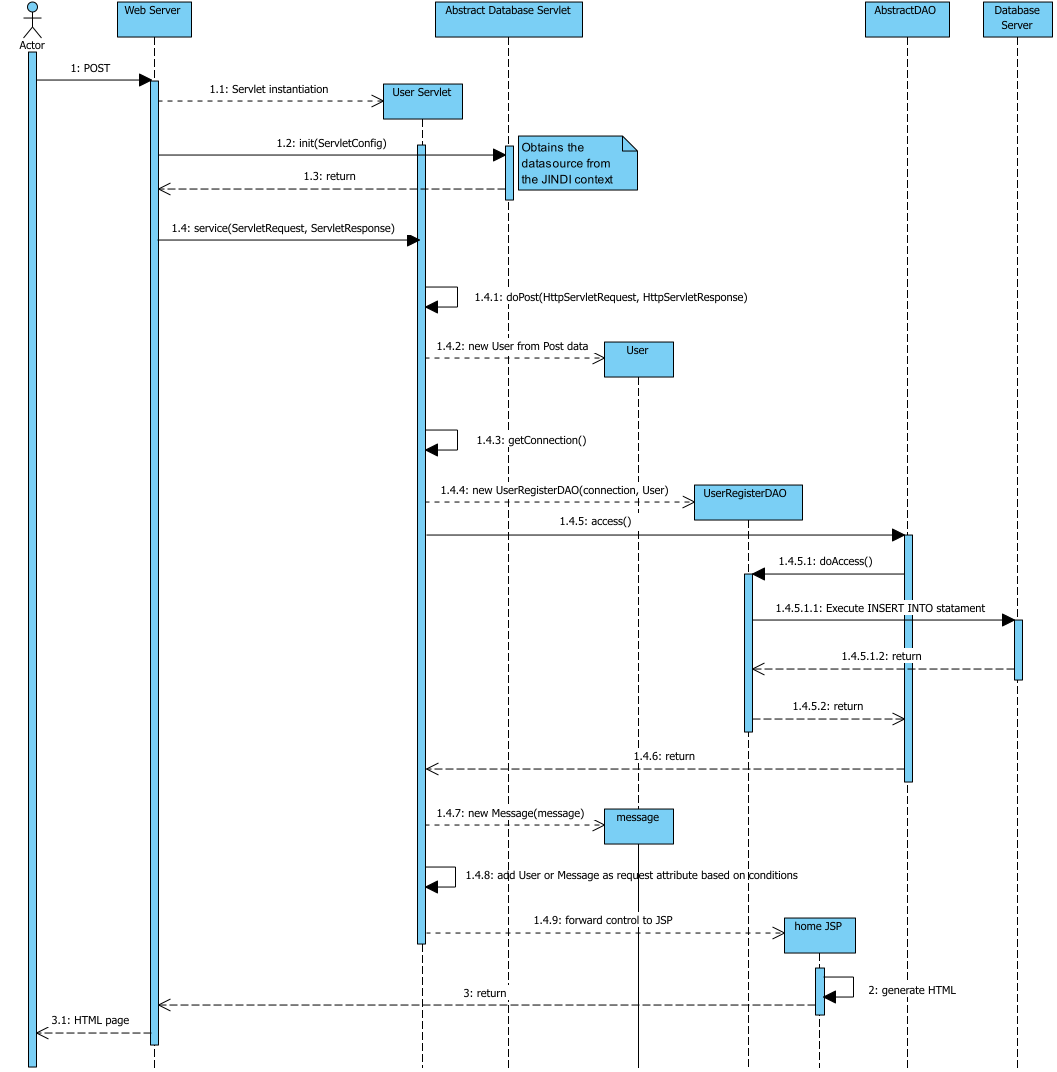
\includegraphics[width=\textwidth]{mockup/InsertUserDiagram}
    \caption{Insert User Sequence Diagram.}
    \label{fig:insertuser}
\end{figure}

One of the basic functionalities of WaCar web application is to give the possibility to not registered user to see which brand and model of cars are available.
The page List Circuit is also capable of dynamically adapt based on the fact of the type of user logged such that if the latter is an \texttt{ADMIN} it gives
the possibility to modify the information about the Car or eventually delete it. The sequence diagram in shown in Fig. \ref{fig:listcircuit} exploits the steps done
via the REST implementation of the circuit list functionality.

\begin{figure}[h]
    \centering
    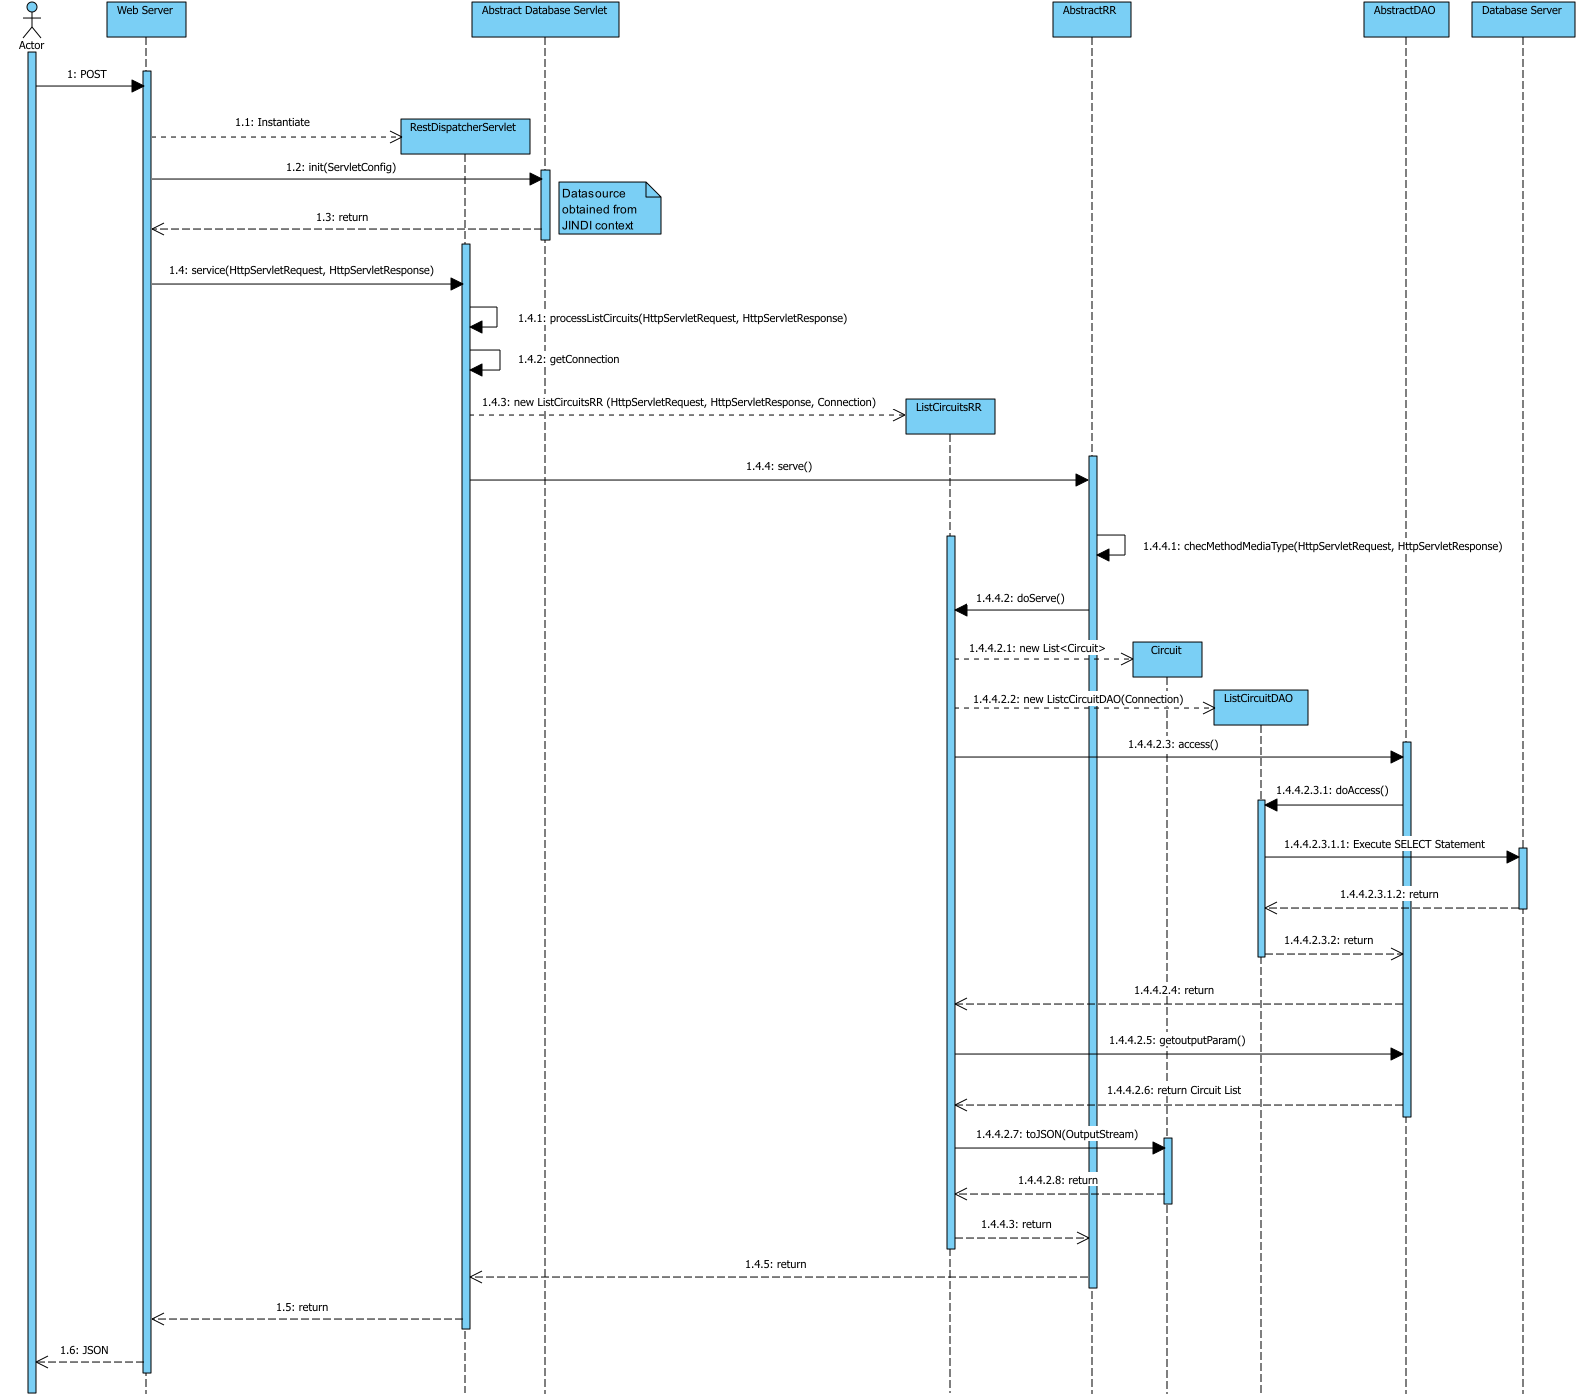
\includegraphics[width=0.8\textwidth]{mockup/ListCircuitsSequenceDiagram}
    \caption{List Circuit REST Sequence Diagram.}
    \label{fig:listcircuit}
\end{figure}

A logged \texttt{USER} has the possibility to review the history of its orders and also manage the one pending in order to eventually modify them. To do so, the user
first needs to log in with its credentials and then access the page \texttt{List Orders}. Upon accessing such page, a \texttt{GET} request is sent to the Web Server
to instantiate the \texttt{ListOrdersByEmailServlet} which then calls its \texttt{doGet()} method and gets the connection to access the database. Afterwards, through
the \texttt{ListOrdersByEmailDAO} class the appropriate \texttt{SELECT} statement is executed to retrieve the data from the database which in this case are the list of orders
related to the specific user sending the request, searched in the database according to the email of the user itself.
In case of errors a \texttt{Message} is instantiated to inform the user, otherwise the results retrieved by the query operation are processed and returned.
The \texttt{ListOrdersByEmailServlet} forwards the control to the \texttt{list-orders} JSP page which generates the HTML document
to display the information to the User.

\begin{figure}[h]
    \centering
    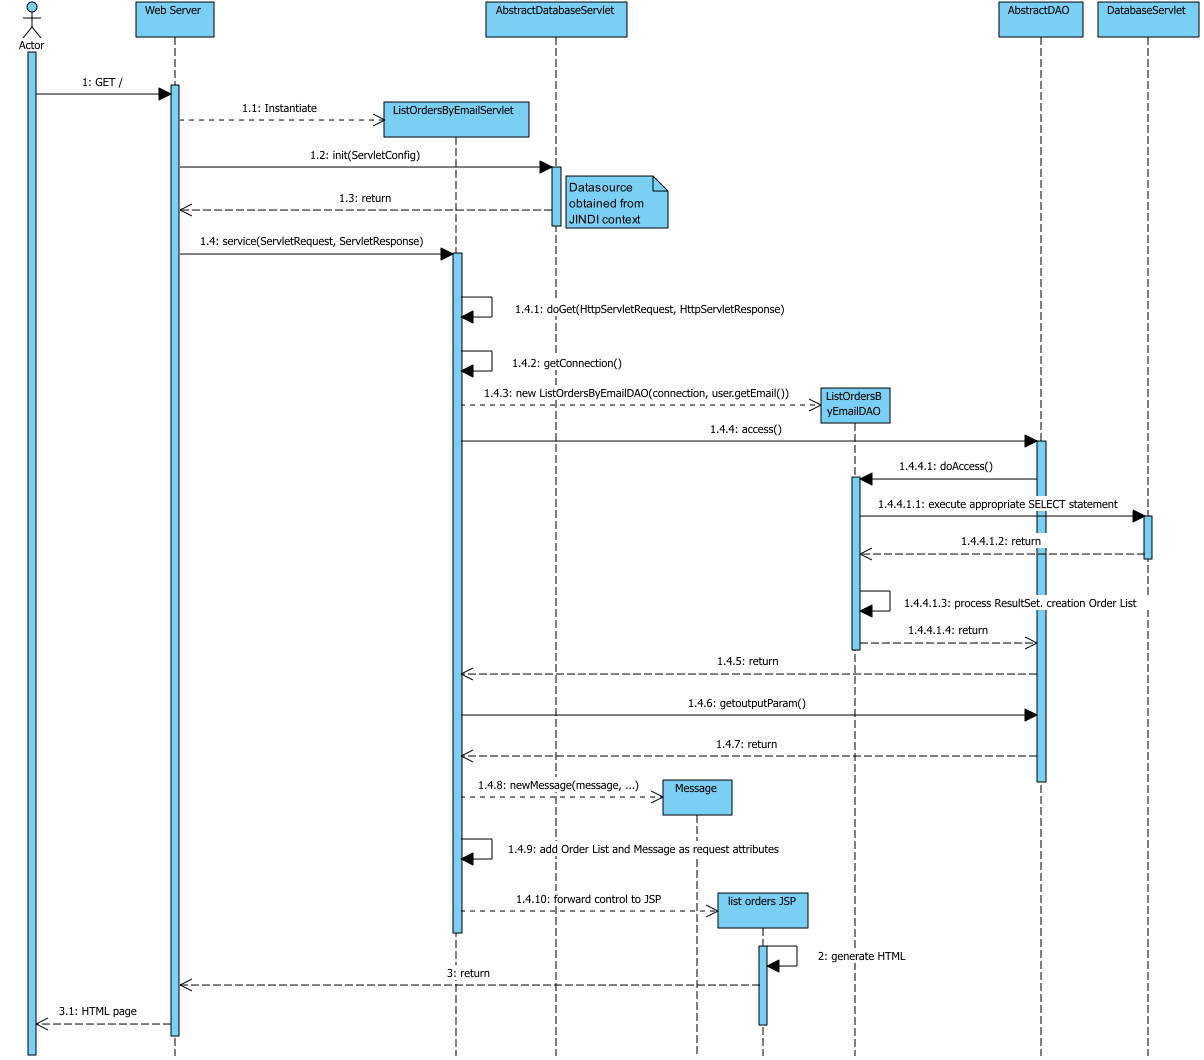
\includegraphics[width=0.8\textwidth]{mockup/ListOrderByEmailSequenceDiagram}
    \caption{List Order by Email Sequence Diagram.}
    \label{fig:listorder}
\end{figure}

\newpage
